\documentclass{beamer}
\usetheme{metropolis}
\usepackage{physics}
\usepackage{ragged2e}
\usepackage{tikz-feynman}
\usepackage{bm}
\usepackage{xcolor}
\usepackage[absolute,overlay]{textpos}

% define  a e s t h e t i c  colors
\definecolor{col1}{HTML}{ef548a}
\definecolor{col2}{HTML}{328eed}
\definecolor{col3}{HTML}{cd665f}
\definecolor{col4}{HTML}{73b517}
\definecolor{col5}{HTML}{6446ad}

\newcommand{\me}{\mathrm{e}}
\newcommand{\mi}{\mathrm{i}}

\title{Final year project presentation\\Neutrino
oscillations and \\experimental sensitivity}
\author{Matthias Dubouchet\\Dr. Lisa Falk}
\date{February 1, 2018}

\begin{document}

\maketitle


\begin{frame}{Outline}

	\begin{itemize}
		\item Neutrinos, neutrino oscillations
		\item Mass hierarchy and CP-violating phase
		\item Experimental sensitivity
	\end{itemize}

\end{frame}


\begin{frame}{What's a neutrino?}

		\begin{itemize}
		\item Lightest lepton
		\item Spin $\frac{1}{2}$ fermion
		\item Interacts only via weak force
		\item Three flavors, produced by corresponding charged current interaction
		\end{itemize}

	\begin{textblock*}{0.6\textwidth}(0.7\textwidth,1.5cm)
		\feynmandiagram [vertical=a to b] {
			e [particle=\(\mu^-\)] -- [fermion] a  -- [fermion] n
			[particle=\(\nu_{\mu}\)],
			 a -- [boson, edge label=\(W^-\)] b,
			};
	\end{textblock*}
\end{frame}


\begin{frame}{Neutrino oscillations: some history}

		\begin{itemize}
			\item Theorized by Bruno Pontecorvo in 1957
			\item Observed by SuperK (1999) and SNO
				(2001)\\\hspace{1cm}$\hookrightarrow$ 2015 Nobel Prize
			\item Implications of the discovery:
				\begin{itemize}
					\item Three neutrinos
					\item Solar neutrino problem solved \checkmark
					\item Beyond the Standard Model physics
				\end{itemize}

		\end{itemize}

\end{frame}


\begin{frame}{Neutrino oscillations}
	\begin{textblock*}{0.6\textwidth}(0.66\textwidth, 1.2cm)
		\includegraphics[width=\textwidth]{bases.pdf}
	\end{textblock*}
	
	\begin{textblock*}{\textwidth}(0.08\textwidth, 0.28\textwidth)
		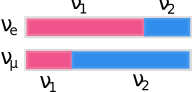
\includegraphics[width=0.2\textwidth]{eigenstates.pdf}
	\end{textblock*}

	\vspace{0.5cm}
	\onslide<1->{
	\begin{itemize}
		\item Mass eigenstates and weak eigenstates
		\item Two neutrinos
	\end{itemize}
	\vspace{-0.5cm}

		$$
			\begin{bmatrix} \nu_e \\ \nu_\mu \end{bmatrix} =
			\begin{bmatrix} \cos\theta & \sin\theta \\
										 -\sin\theta & \cos\theta \end{bmatrix}
				\begin{bmatrix} \nu_1 \\ \nu_2 \end{bmatrix}
			$$
		}
		\onslide<2->{
			\begin{align*}
				&\ket{\psi(0)} = \ket{\nu_e} \equiv \cos{\theta}\textcolor{col1}{\ket{\nu_1}} +
				\sin{\theta}\textcolor{col2}{\ket{\nu_2}}\\[0.2cm]
				&\ket{\psi(\bm{x}, t)} = \cos{\theta} \textcolor{col1}{\ket{\nu_1}
				\me^{-\mi p_1 \cdot x}} +
				\sin{\theta} \textcolor{col2}{\ket{\nu_2} \me^{-\mi p_2 \cdot
				x}}\\[0.3cm]
				&\hspace{0.5cm}P(\nu_{e}, \bm{X}, T) =
				|\bra{\nu_{e}}\ket{\psi(\bm{X}, T)}|^2 \textcolor{col3}{\neq
				1}
			\end{align*}
		Different masses $\rightarrow$ different phases $\rightarrow$ flavor oscillations
		}
	\onslide<3->{
	$$P(\nu_e, \bm{X}, T) = \sin^2 2\theta~ \sin^2 \frac{\Delta m^2 L}{4 E}$$
	}
	\pause

	\begin{textblock*}{0.65\textwidth}(0.4\textwidth,1.7cm)
	\includegraphics<3->[width=\textwidth]{twonu4.pdf}
	\end{textblock*}


\end{frame}
	

\begin{frame}{Three neutrino case}

	 
	\begin{textblock*}{\textwidth}(0.5cm,1.5cm)
		\onslide<+->{
		$$
		\begin{bmatrix} \nu_e \\ \nu_\mu \\ \nu_\tau \end{bmatrix} = 
			\begin{bmatrix} 1 & 0 & 0 \\ 0 & \textcolor{col1}{c_{23}} &
			\textcolor{col1}{s_{23}} \\ 0 & -\textcolor{col1}{s_{23}} &
			\textcolor{col1}{c_{23}} \end{bmatrix}
		\begin{bmatrix} \textcolor{col2}{c_{13}} & 0 & \textcolor{col2}{s_{13}}
			\me^{-\mi \textcolor{col5}{\delta_{CP}}} \\ 0 & 1 & 0 \\
		-\textcolor{col2}{s_{13}} \me^{\mi \textcolor{col5}{\delta_{CP}}} & 0 &
		\textcolor{col2}{c_{13}} \end{bmatrix} 
		\begin{bmatrix} \textcolor{col4}{c_{12}} & \textcolor{col4}{s_{12}} & 0 \\
		-\textcolor{col4}{s_{12}} & \textcolor{col4}{c_{12}} & 0 \\ 0 & 0 & 1 \end{bmatrix}
		\begin{bmatrix} \nu_1 \\ \nu_2 \\ \nu_3 \end{bmatrix}
		$$
		$$\textcolor{col1}{c_{23}} = \cos{\textcolor{col1}{\theta_{23}}}, \quad
		\textcolor{col4}{s_{12}} = \sin{\textcolor{col4}{\theta_{12}}}, \quad
		...$$
		}

		\onslide<+->{
			\vspace{-0.5cm}
			\hspace{0.7cm}$\rightarrow$ Three mixing angles (Euler angles),
			one imaginary phase

		\vspace{0.5cm}
		$$
			P(\nu_\alpha \rightarrow \nu_\beta) \propto \sum_{i j} \exp(-i
			\frac{\Delta m^2_{i j} L}{2 E}) \qquad \qquad \Delta m^2_{ij} = m^2_i - m^2_j
		$$}
	\end{textblock*}
	
	\begin{textblock*}{0.9\textwidth}(0.15\textwidth,1.1cm)
		\includegraphics<+->[width=0.95\textwidth]{threenu.pdf}
	\end{textblock*}

\end{frame}

\begin{frame}{The mass ordering}

	\vspace{1cm}
	\begin{itemize}
		\item An extra ambiguity
	\end{itemize}

	\vspace{-0.5cm}
	%\begin{textblock*}{0.8\textwidth}(0.15\textwidth,1.1cm)
		\includegraphics[width=\textwidth]{hierarchy.pdf}

	%\end{textblock*}

\end{frame}


\begin{frame}{The importance of parameters}

	\begin{textblock*}{\textwidth}(0.1\textwidth,1.8cm)
		\includegraphics<+->[width=0.75\textwidth]{parameters_d.pdf}
	\end{textblock*}
	\begin{textblock*}{\textwidth}(0.4\textwidth, 4cm)
	\includegraphics<+->[width=0.75\textwidth]{parameters_mh.pdf}
	\end{textblock*}

\end{frame}


\begin{frame}{Matter effects}

	\begin{itemize}
		\item Matter is made of electrons
		\item Electron-neutrinos interact with electrons!
	\end{itemize}
	% forward scattering in matter
	% effective mass
	% impact on transition probability
	%\begin{textblock*}{0.65\textwidth}(0.05\textwidth,5.1cm)
		\includegraphics[width=0.85\textwidth]{matter.pdf}
	%\end{textblock*}

\end{frame}


\begin{frame}{Sensitivity}

	\begin{itemize}
		\item Can we know whether a future experiment will yield useful results?
		\item How much data would we need to be able to draw sensible conclusions?
		\item Define \emph{sensitivity} statistic: 
			$$\overline{\Delta \chi^2} = \sum_i \frac{(y^A_i - y^B_i)^2}{\sigma^2_i}$$

	\end{itemize}

\end{frame}


\begin{frame}{Sensitivity}

	\begin{textblock*}{\textwidth}(1cm, 8.5cm)
		\footnotesize{
			$$\overline{\Delta \chi^2} = \sum_i \frac{(y^A_i - y^B_i)^2}{\sigma^2_i}$$
			}
	\end{textblock*}

	\begin{textblock*}{\textwidth}(1cm, 1.3cm)
	\onslide<+->{
		Sensitivity to the mass hierarchy\\\vspace{0.2cm}
		\includegraphics[width=0.9\textwidth]{sens.pdf}}\\
	\end{textblock*}
	
	\begin{textblock*}{\textwidth}(2.5cm, 4cm)
	\onslide<+->{
	\includegraphics[width=0.9\textwidth]{sens_cp.pdf}\\
		\vspace{-1.7cm}\hspace{5cm}Sensitivity to the \\\hspace{5cm}CP violating phase}
	\end{textblock*}

\end{frame}


\begin{frame}{What's next}

	\begin{itemize}
	\item Introduce randomness in the model
	\item 
	\end{itemize}

\end{frame}


\begin{frame}{Summary}


\end{frame}

\begin{frame}{References}

	\scriptsize{
	\begin{itemize}
		\item Zuber, K. (2004). \emph{Neutrino Physics}
		\item Thomson, M. (2013). \emph{Modern Particle Physics}
		\item Ciuffoli, Evslin, Zhang (2013). \emph{Sensitivity to the Neutrino
			Mass Hierarchy}
			(1305.5050)
		\item NOvA Collaboration (2017). \emph{Constraints on Oscillation Parameters from
			$\nu_e$ Appearance and $\nu_\mu$ Disappearance in NOvA} (1703.03328)
		\item DUNE Collaboration (2015). \emph{Long-Baseline Neutrino Facility (LBNF) and
			Deep Underground Neutrino Experiment (DUNE) Conceptual Design Report}
		\item Kayser, B. (2008), \emph{Neutrino Oscillation Phenomenology} (0804.1121)
		\item Qian, Tan, Wang, Ling, McKeown, Zhang (2012). \emph{Statistical Evaluation of
			Experimental Determinations of Neutrino Mass Hierarchy} (1210.3651)
		\item Smirnov, A. (2004), \emph{The MSW effect and Matter Effects in Neutrino
			Oscillations} (04122391)
		\item Blennow, M. (2015), \emph{Mass hierarchy sensitivity at future
			oscillation facilities}
	\end{itemize}}

\end{frame}



\end{document}
